%!TEX root = ../paper.tex

% ---------------------------------------------------------------------------- %
% Outline

\iftoggle{outline}{
    \begin{itemize}
        \item Progress so far
        \item Diagram of components
        \item Benchmarks and description
    \end{itemize}
}

\iftoggle{oldcomments}{
    \mwh{It would be good to say which functionalies are supported so far, and how those were selected (because they matched what SOMns already does? because they matched existing Grace benchmarks?). That may affect how any metric results should be interpreted.}
}

% 
% ---------------------------------------------------------------------------- %

Reusing an existing Grace parser, we translate Grace's \AST/ nodes into those used by SOMns to have a basic Grace \VM/, see \autoref{fig:components}.
Thus, we modified SOMns to use our translator. When called, the translator first parses Grace's prelude and then continues to the input program.
Once an \AST/ has been formed, the translator composes the program representation based on SOMns's Truffle nodes. 

\begin{figure}
    \centering
    \makebox[\columnwidth][c]{
        \resizebox{\columnwidth}{!}{
            
\begin{tikzpicture}[
	edge from parent/.style ={}
]

\node[obselete] (NewspeakPrelude) {Newspeak Prelude};
\node[obselete, xshift=2cm, right of = NewspeakPrelude] (NewspeakParser) {Newspeak Parser};

\node[exists, xshift=2cm, right of = NewspeakParser] (SOMnsAST) {SOMns AST};
\node[exists, xshift=2cm, right of = SOMnsAST] (Truffle) {Truffle};
\node[exists, xshift=2cm, right of = Truffle, below of = Truffle] (Graal) {Graal};

\node[created, yshift=-1cm, below of = SOMnsAST] (Translator) {Translator};
\node[exists, yshift=-1cm, below of = Translator] (GraceAST) {Grace AST};
\node[exists, xshift=-2cm, left of = GraceAST] (GraceParser) {Grace Parser};
\node[exists, xshift=-2cm, left of = GraceParser] (GracePrelude) {Grace Prelude};


\draw[->>, dashed] (NewspeakPrelude) -- (NewspeakParser);
\draw[->>, dashed] (NewspeakParser) -- (SOMnsAST);
\draw[->>, thick] (SOMnsAST) -- (Truffle);
\draw[->>, thick] (Truffle) |- (Graal);
\draw[->>, thick] (Graal) |- (Truffle);

\draw[->>, thick] (GracePrelude) -- (GraceParser);
\draw[->>, thick] (GraceParser) -- (GraceAST);
\draw[->>, thick] (GraceAST) -- (Translator);

\draw[->>, thick] (Translator) -- (SOMnsAST);

\end{tikzpicture}
        }
    }
    \caption{SOMns is built upon Truffle and Graal and implements an \AST/ for Newspeak. We parse programs written in Grace using an existing parser, and translate the generated nodes into those used by SOMns.}
    \label{fig:components}
\end{figure}

For the initial proof of concept, we implemented expression nodes, numerals and string nodes, as well as nodes to maintain lexical scoping for blocks and methods. The translator is little more than an AST visitor that reads the nodes in one form and exports them in other; and in a few cases it composes together multiple nodes to preserve Grace's semantics. 

\begin{figure}
    \centering
    \makebox[\columnwidth][c]{
        \resizebox{\columnwidth}{!}{
            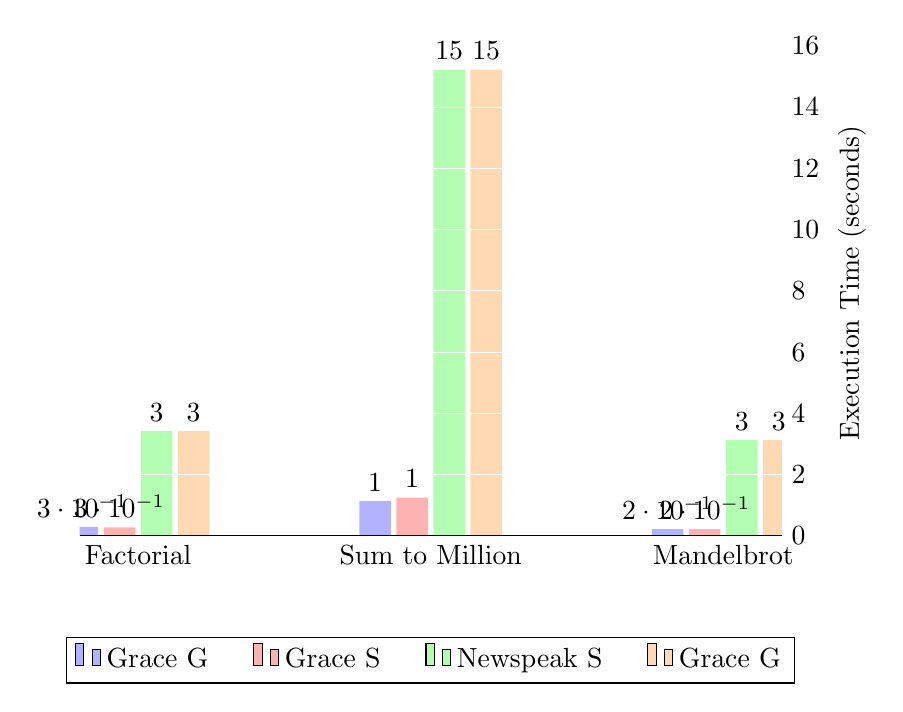
\begin{tikzpicture}
    \begin{axis}[
        ybar, axis on top,
        height=8cm, width=10.5cm,
        bar width=0.4cm,
        ymajorgrids, tick align=inside,
        major grid style={draw=white},
        enlarge y limits={value=.1,upper},
        ymin=0, ymax=15,
        axis x line*=bottom,
        axis y line*=right,
        y axis line style={opacity=0},
        tickwidth=0pt,
        enlarge x limits=true,
        legend style={
            at={(0.5,-0.2)},
            anchor=north,
            legend columns=-1,
            /tikz/every even column/.append style={column sep=0.5cm}
        },
        ylabel={Execution Time (seconds)},
        symbolic x coords={
           Factorial,
           Sum to Million,
           Mandelbrot},
       xtick=data,
       nodes near coords={
        \pgfmathprintnumber[precision=0]{\pgfplotspointmeta}
       }
    ]
    \addplot [draw=none, fill=blue!30] coordinates {
      (Factorial, 0.294)
      (Sum to Million, 1.132)
      (Mandelbrot, 0.224) };
    \addplot [draw=none,fill=red!30] coordinates {
      (Factorial,0.274)
      (Sum to Million, 1.253) 
      (Mandelbrot, 0.223)  };
    \addplot [draw=none, fill=green!30] coordinates {
      (Factorial, 3.431)
      (Sum to Million,  15.223) 
      (Mandelbrot, 3.129) };
    \addplot [draw=none, fill=orange!30] coordinates {
      (Factorial, 3.431)
      (Sum to Million,  15.223) 
      (Mandelbrot, 3.129) };

    \legend{Grace G, Grace S, Newspeak S, Grace G}
    \end{axis}
\end{tikzpicture}
        }
    }
    \caption{Average execution time when executing three benchmarks, implemented equvilantely in both Grace and Newspeak. Results with and without the Graal optimization layer are presented.}
    \label{fig:benchmark}
\end{figure}

Despite being tailored to Newspeak, SOMns can be easily adapted to Grace through our translator. To date SOMns has been under development for $22$ months: it is mostly compliant with Newspeak, and is as fast as other \JITing/ \VMs/. In contrast Grace has been in development for around five years, without consideration of performance. In only three weeks, we have adapted a Truffle-based \VM/ to realize a new implementation that supports Grace's numeral and string literals, nesting of blocks, method and field declarations, and object and class instantiation and nesting with compliance to the Grace specification\footnotemark. \rr{Is what I say here true?} With the implmentation, Grace programs can be executed with comparable speed to Newspeak. As demonstrated in \autoref{fig:benchmark}, there is only a marginal loss of performance due to the additional translation step. In conclusion, the implementation retains much of the optimizations carefully tailored for Newspeak and required only a trivial amount of work.

\footnotetext{\url{http://gracelang.org/documents/grace-spec-0.7.0.pdf}}


% We have presented an experiment in which we realized a \VM/ for Grace from SOMns, while retaining much of the \AST/ optimizations. While further experiments are required before we can quantify the extent to which the similarity of the languages, the craft of SOMns, and the flexibility of Truffle contribute to the ability to make such an adaption.\mwh{While further experiments are required, what?} 
